\chapter{OBJECT DETECTION}

\renewcommand{\headrulewidth}{0.5pt}
\renewcommand{\footrulewidth}{0.5pt}
\thispagestyle{plain}
\pagestyle{fancy}
\fancyhf{}
\fancyhead[L]{\textbf{CHAPTER 2}}
\fancyhead[R]{\textbf{Intelligent Traffic System}}
\raggedright
\fancyfoot[L]{From: ITM Vision}
\fancyfoot[R]{Page \thepage}

\section{Overview}

    \subsection{Traditional Methods}
        Traditional object detection methods are built on handcrafted features and shallow trainable architectures. \\
        \vspace{3mm}
        Features used in traditional methods: color feature, HOG feature, edge feature, optical flow features, texture features,... \\
        \vspace{3mm}
        The pipeline of traditional object detection models can be mainly divided into three stages: informative region selection, feature extraction, and classification.
    
    \subsection{Deep Learning Based Method}

        \subsubsection{ANN}
            An ANN consists of interconnected groups of nodes. Each group is called a layer and
            each node is called a neuron. The connection between neurons, replicating synapses
            in biological brains, transfers information between layers. A very simple ANN can be
            seen in where two inputs are going through a hidden layer in order to produce an output.    
            \begin{figure}[H]
                \centering
                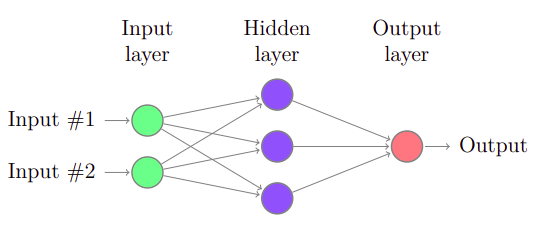
\includegraphics[width=0.6\linewidth]{img/ANN.png}
                \caption{Example of an Artificial Neural Network with two input, one hidden and output layer}
            \end{figure}
        
        \subsubsection{Neurons}
            The artificial neurons in neural networks is a mathematical model of a biological
            neuron, modelled to replicate the function of being excitable depending on input
            signals. The equation of a neuron, visualized as one of the blue circles,
            is simply a weighted sum of all the inputs plus a bias term, i.e.
            \begin{align}
                s(x) = \displaystyle\sum_{i=0}^n w_i x_i + b_i
            \end{align}
            \vspace{3mm}
            where \emph{n} is the number of inputs and \emph{$w_i$} the weights in the neuron and \emph{$b_i$} 
            the bias term. The combination of weights and input signals, giving the neuron its value
            together with the bias term, represents the excitability.

        \subsubsection{Activation Functions}
            The activation functions are essential components of ANNs, used to perform nonlinear mappings of the input data and are typically applied element-wise to all
            neurons in a hidden layer. This section describes a few commonly used activation
            functions and their properties. The activation functions commonly used in the
            intermediate layers of ANNs are presented.
            \begin{figure}[H]
                \centering
                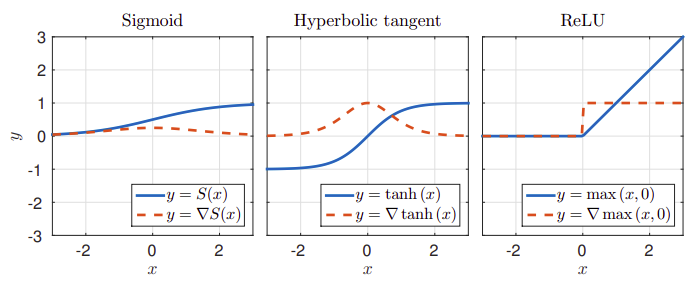
\includegraphics[width=0.6\linewidth]{img/sigmoid.png}
                \caption{The sigmoid, hyperbolic tangent and ReLU activation functions and
                their derivatives}
            \end{figure}
            \begin{enumerate}
                \item \textbf{Sigmoid} \\ 
                    \vspace{3mm}
                    The sigmoid activation functions is defined as: 
                    \begin{align}
                        S(x) = \frac{1}{1 + e^{-x}}
                    \end{align}
                    It takes values from 0 to 1 and is linear close to the origin. It has a "squashing" 
                    property such that large positive or negative input values result in values close to 1
                    or 0 respectively.
                \item \textbf{Hyperbolic Tangent} \\ 
                    \vspace{3mm}
                    The hyperbolic tangent: 
                    \begin{align}
                        tan(x) = \frac{sin(x)}{cos(x)} = \frac{e^x - e^{-x}}{e^x + e^{-x}}
                    \end{align}
                    is also commonly used as activation function in ANNs. It has very similar properties
                    to the sigmoid function except tan(x) takes values from −1 to 1.
                \item \textbf{Rectified Linear Unit} \\ 
                    \vspace{3mm}
                    The Rectified Linear Unit (ReLU) is an activation function commonly used with
                    deep neural networks, and is simply given by:
                    \begin{align}
                        f(x) = max(x,0)
                    \end{align}
                    Compared to the commonly used sigmoid activation function, the ReLU has the
                    advantage of not saturating for large inputs. While sigmoidal functions take values
                    in the range (0, 1), ReLUs take values in 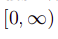
\includegraphics[scale=0.4]{img/range.png} making them less prone to be either
                    “on” or “off”.
                \item \textbf{Softmax} \\ 
                    \vspace{3mm}
                    The softmax function is a normalising function commonly used as an activation
                    function for the last layer of a neural network. Given an input vector \emph{x} 
                    with values \emph{$x_i$}, the corresponding output element \emph{$y_i$} is calculated.
                    \begin{align}
                        y_i = \frac{e^{x_i}}{\displaystyle\sum_{j=1}^N e^{x_j}}
                    \end{align}
                    By construction, the elements of the output vector sums to 1. This property is useful
                    when the output of the neural network should encode probabolities for different
                    cases, such as in classification tasks.
            \end{enumerate}

        \subsubsection{Convolution Neural Networks}
            Convolutional Neural Networks (CNNs) are feedforward neural networks with a
            layout and architecture specifically designed to handle data arranged in a spatial
            grid (tensors), such as 2D or 3D images. The inspiration of the architecture comes
            from the mechanism of biological visual perception. The networks, like any other
            ANN, are composed of neurons with learnable weights and biases. Each neuron
            receives some inputs, performs a dot product and optionally follows it with an
            activation function. The architecture is typically composed of several layers, which
            gives them the characterisation of being “deep” and thus research work on CNNs fall
            under the domain of deep learning. Essentially, the network computes a mapping
            function that relates image pixels to a final desired output. \\ 
            \vspace{3mm}
            In a general CNN, the input is assumed to be an RGB image, i.e. consisting of
            three channels, corresponding to the red, green and blue color intensity values.
            Consecutive layers of the CNN may consist of even more channels referred to as
            \emph{feature maps}. The number of feature maps typically increase through the layers of
            a CNN, while the spatial dimension of them decreases until reaching the desired
            output size. The over-all idea behind this structure is that the representation of the
            input image is gradually increased in abstraction as it progresses through the layers.
            Later layers contain more information about the “what” and “how” of objects and
            things in an image, and less of “where”. Similar to the definition of a feature map,
            a \emph{feature vector} at a specific layer of a CNN is defined to be the elements across all
            feature maps at a given spatial location. An example of the structure of a CNN is
            presented. 
            \begin{figure}[H]
                \centering
                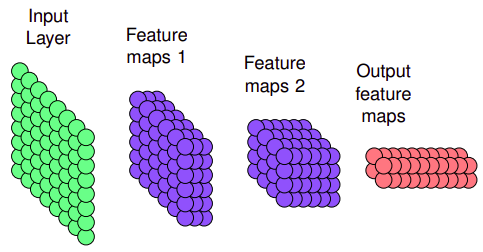
\includegraphics[width=0.6\linewidth]{img/illustration.png}
                \caption{Illustration of how neurons are structured in a CNN}
            \end{figure}
            \begin{enumerate}
                \item \textbf{Components of CNNs} \\ 
                    \vspace{3mm}
                    Besides the fully connected layer presented in, there are other types of
                    layers and connections that can be used to construct deep convolutional networks.
                    Typically, the purposes behind some of these components are to reduce the dimensions of intermediate layers, reshaping spatial dimensions, simulating fully connected
                    layers and more. Following are some sections describing important components in
                    the CNN framework used in this thesis. \\ 
                    \vspace{3mm}
                    \ding{114}\textbf{Convolution} \\ 
                    \vspace{3mm}
                    The discrete 2D convolution operation, is defined by a convolution kernel \emph{k} of size 
                    \emph{k x k}. Given an \emph{N x M} input image (tensor) \textbf{X}, the convolution kernel is run along all the pixels in the image, multiplying the
                    surrounding pixel values with the kernel and adding them. The resulting output is
                    a \emph{(N -k +1) x (M - k -1)} image \textbf{Y}, where the output at pixel location \emph{i,j} is calculated: 
                    \begin{align}
                        Y_{i,j} = \displaystyle\sum_{i'=1}^k \displaystyle\sum_{j'=1}^k k_{i',j'} X_{\frac{i - (k+1)}{2+j'}, \frac{j-(k+1)}{2+j'}}
                    \end{align}
                    The operator is denoted using * and thus 
                    \begin{align}
                        Y = k*X
                    \end{align}
                    \begin{figure}[H]
                        \centering
                        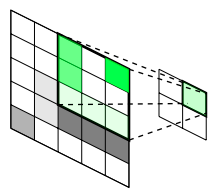
\includegraphics[width=0.4\linewidth]{img/conv_operation.png}
                        \caption{Illustration of the convolution operation using a 3 x 3 kernel}
                    \end{figure}
                    The convolution operation between two layers in a CNN is defined by a kernel \textbf{$k_{ij}$} for each pair of feature maps in the two layers. Similar to the fully connected layer,
                    the result from all convolutions related to feature map \emph{i} in the later layer is summed
                    and a bias $b_i$ is distributed and added across the entire feature map. Let \textbf{$X_j$}, be a feature map in a layer with N$\geq$j features maps, then the feature map \textbf{$Y_i$} in 
                    the next layer is calculated
                    \begin{align}
                        Y_i = \sigma_i (\displaystyle\sum_{j=1}^N k_{ij} * X_j + b_i 1)
                    \end{align}
                    where \textbf{1} is an all-ones matrix and $\sigma_i$
                    is an element-wise activation function. The
                    elements of all kernels \textbf{$k_{ij}$} and the biases \emph{$b_i$} are learnable parameters and are updated
                    through the process of training the network. \\ 
                    \vspace{3mm}
                    As mentioned, the convolution operation has the effect of reducing the dimensions
                    of the feature maps. However, there are some methods which can be used to avoid
                    or modify this effect. A common strategy to preserve the spatial dimensions is to
                    apply zero-padding, i.e. covering the feature maps before the convolution operation
                    with a border of $\frac{k-1}{2}$ zeros, which counters the spatial reduction exactly. On
                    the other hand, to reduce the spatial dimensions of intermediate layer activations
                    further, a \emph{stride} can be associated with the convolution. The stride is applied by
                    sliding the convolution kernel by \emph{s} number of steps between each “multiply and
                    sum” operation and the result is that the feature maps are reduced in size by a
                    factor \emph{s}. Most commonly, the convolutions are applied without stride, i.e. s = 1. \\ 
                    \vspace{3mm}
                    An important concept introduced by applying a convolution layer to a CNN is the
                    \emph{receptive field}. The receptive field is a measure of how much information from the
                    input image is available to the feature vectors of a specific layer in a CNN. If the
                    first component of a CNN is a convolutional layer with kernel width \emph{$k_1$}, the receptive
                    field of the first layer is k1 x k1 – i.e. each element in the second layer was provided
                    information from the k1×k1 nearest pixels in the input image. Following this pattern,
                    a series of n convolution layers with kernel sizes \emph{$k_1, . . . , k_n$} results in a receptive field
                    of
                    \begin{align}
                        (1 + \displaystyle\sum_{i=1}^n (k_i - 1)) \times (1 + \displaystyle\sum_{i=1}^n (k_i - 1))
                    \end{align}
                    \ding{114}\textbf{Up-convolution or backwards convolution} \\ 
                    \vspace{3mm}
                    An operation analogous to the convolution operation, but reversed, referred to as
                    up-convolution can be used for upsampling. It is achieved by convolution operation
                    reversed. Hence, if upsampling by a factor \emph{f} is desired, it
                    can be formulated as a convolution with a fractional input stride of $\frac{1}{f}$. Such 
                    a layer can associate a single input activation to multiple output activations. This "upconvolution" layer has learnable filter parameters that could correspond to bases
                    for reconstructing shapes of an object. Hence, an end-to-end learning mechanism can be constructed by repeated downsampling and then upsampling to achieve
                    dense predictions, and this technique has been successfully used for dense pixel-level
                    predictions.
                    \begin{figure}[H]
                        \centering
                        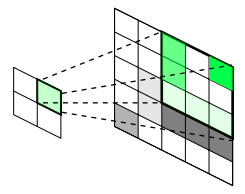
\includegraphics[width=0.4\linewidth]{img/up-convolution.png}
                        \caption{Illustration of the upconvolution operation}
                    \end{figure}
                    \ding{114}\textbf{Pooling} \\ 
                    \vspace{3mm}
                    Pooling layers are non-learnable layers used to reduce the spatial dimensions of the
                    feature maps as they pass through the network. Similar to the convolution layer,
                    they are associated with some kernel of size \emph{k x k} and a stride \emph{s}. There are two
                    commonly used types of pooling layers; the max-pooling layer and the averagepooling layer. The max-pooling layer,performs a max ()
                    operation with the elements of the feature map at each position of the kernel, thus
                    discarding the information of the non-max neurons.
                    \begin{figure}[H]
                        \centering
                        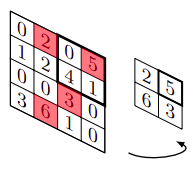
\includegraphics[width=0.4\linewidth]{img/max-pooling.png}
                        \caption{Illustration of the max-pooling operation}
                    \end{figure}
                    The average-pooling layer performs an average at each position of the kernel, i.e. a
                    normal convolution with the kernel values all set to $\frac{1}{k^2}$. Typically, the stride of
                    the pooling layers is set to \emph{s=k} , thus achieving a dimensional reduction of a factor
                    \emph{s} without using any zero-padding. \\ 
                    \vspace{3mm}
                    Apart from reducing the spatial dimensions of the feature maps, pooling layers also
                    provide an efficient way of increasing the receptive field in a CNN. A pooling layer
                    with stride \emph{s} have the effect of increasing the receptive field of a factor \emph{s}. This effect
                    can also we achieved by including stride in a convolutional layer. \\ 
                    \vspace{3mm}
                    \ding{114}\textbf{Unpooling} \\ 
                    \vspace{3mm}
                    A reverse operation to pooling, “unpooling” aims to recover the original size of activations that were lost due to a pooling operation. A version of unpooling specifically
                    for reversing the max-pooling operation, records the maximum activations selected
                    during the pooling operation and uses them to recreate the original activations by
                    placing the recorded values in their original positions. This strategyis useful to recover the structure of objects and have a parameter-free
                    upsampling. 
                    \begin{figure}[H]
                        \centering
                        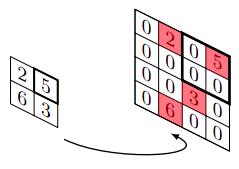
\includegraphics[width=0.4\linewidth]{img/max-unpooling.png}
                        \caption{Illustration of the max-unpooling operation}
                    \end{figure}
                    \ding{114}\textbf{1 x 1 Convolutions} \\ 
                    \vspace{3mm}
                    Technically, 1 × 1 convolutional kernels are no different from any k × k kernel in the
                    way they are applied. However, there is a conceptual difference between them in
                    that k × k convolutions are usually thought of as edge/feature detectors while 1 × 1
                    kernels can only combine activations of each feature vector. The interpretation of
                    such an operation is that it is simulating the effect of a fully connected layer, applied
                    to each feature vector. Since the convolution operation is not dependant on the
                    spatial size of its input, transforming fully connected layers to 1 × 1 convolutions is
                    a useful way of generalizing the network for different input sizes. \\ 
                    \vspace{3mm} 
                    \ding{114}\textbf{Batch Normalisation} \\ 
                    \vspace{3mm}
                    Training deep neural networks can be quite tricky in practice due to the fact that
                    the distribution of each intermediate layer’s inputs changes during training. Such a
                    change is caused by the changes in the parameters of the previous layers. This problem is referred to as \emph{internal covariate shift}. When the input distribution changes,
                    the activations tend to move into the saturated regimes, and this effect is amplified
                    as the network depth increases, thus also causing the vanishing gradient problem.
                    To tackle this, a normalisation technique was introduced, where normalisation of the inputs to the activation layers are done over the mini-batch. The batch
                    normalising transform algorithm is briefly presented. Consider a mini-batch of \emph{n} inputs in a mini-batch \textbf{$\beta = \{x_1,x_2,...,x_n\}$}. Let 
                    the normalized values be $\{\hat{x_1},\hat{x_2},...,\hat{x_n}\}$ and the resulting linear transformation of the batch 
                    normalisation can be represented by $\{y_1,y_2,...,y_n\}$. Then, the batch normalising transform given by 
                    \begin{align}
                        \textbf{BN}_{\gamma,\beta} : \{x_1,x_2,...,x_n\} \rightarrow \{y_1,y_2,...,y_n\}
                    \end{align}
                    where $\gamma$ and$\beta$ are learnable parameters that correspond to the scaling and shifting
                    in the transformation. Hence the mini-batch mean and variance which are given by 
                    \begin{align}
                        \mu \beta \leftarrow \frac{1}{n} \displaystyle\sum_{i=1}^n x_i \\
                        \sigma_\beta^2 \leftarrow \frac{1}{n} \displaystyle\sum_{i=1}^n (x_i - \mu \beta)^2
                    \end{align}
                    are used to achieve the normalisation. Thus, the normalisation looks like
                    \begin{align}
                        \hat{x}_i \leftarrow \frac{x_i - \mu \beta}{\sqrt{\sigma_\beta^2 + \in}}
                    \end{align}
                    and the resulting transformation can be given by
                    \begin{align}
                        y_i \leftarrow \gamma \hat{x}_i + \beta
                    \end{align}
            \end{enumerate}
        \subsubsection{Spped/Accuracy Trade-offs}
            The relation between these two is very complex, as it is very hard to maintain them both
            at a high level. In the case of real-time environment where the focus is on Advanced
            driver-assistance systems (ADAS), a decision needs to be made fast, and by that means
            that the detection of pedestrians and vehicle needs to be fast. In a trade-off there are two
            alternatives, decisions are made fast which results to higher error-rate or slow which then
            results in higher accuracy.
            \begin{figure}[H]
                \centering
                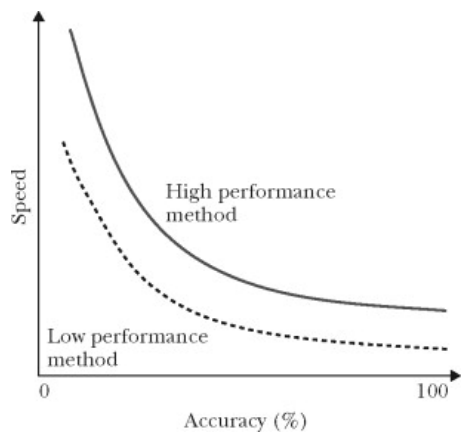
\includegraphics[width=0.6\linewidth]{img/trade-off.png}
                \caption{Speed/Accuracy trade-of}
            \end{figure}
            As shown above, the performance of each axis depend on the other, so if speed
            decreases than the accuracy increases. The trade-off between speed and accuracy needs
            both at a balanced level, otherwise it will be fast with weak detection or good detection
            with low speed. The trade-off between speed and accuracy needs to be at a balanced
            level.

        \subsubsection{Categorize}
            Thanks to Deep Neural Network, a more significant gain is obtained with the introduction of regions with convolutional neural network (CNN) features (R-CNN). DNNs, or the most representative CNNs, act in a quite different way from traditional approaches. They have deeper architectures with the capacity to learn more complex features than the shallow ones. Also, the expressivity and robust training algorithms allow to learn informative object representations without the need to design features manually. \\
            \vspace{3mm}
            Since the proposal of R-CNN, a great deal of improved models have been suggested, including fast R-CNN that jointly optimizes classification and bounding box regression tasks, faster R-CNN that takes an additional subnetwork to generate region proposals, and you only look once (YOLO) that accomplishes object detection via a fixed-grid regression. \\

        \subsubsection{Region Proposal Based Method}
            Generate region proposals at first and then classify each proposal into different object categories. Frameworks may be included such as: R-CNN, Faster R-CNN, region-based fully convolutional network R-FCN, feature pyramid networks (FPN), and Mask R-CNN. \\
            \vspace{3mm}
            Region proposal-based frameworks are composed of several correlated stages, including region proposal generation, feature extraction with CNN, classification, and bounding box regression, which are usually trained separately. Even in the recent end-to-end module Faster R-CNN, an alternative training is still required to obtain shared convolution parameters between RPN and detection network. As a result, the time spent in handling different components becomes the bottleneck in the real-time application. \\

        \subsubsection{Regression / Classification Based Method}
            Regression/classification based framework solves object detection problem by regarding it as regression or classification problem. Some frameworks may be accounted for examples are: MultiBox, AttentionNet, G-CNN, YOLO, Single Shot MultiBox Detector (SSD), YOLOv2, YOLOv3. \\
            \vspace{3mm}
            One-step frameworks based on global regression/classification, mapping straightly from image pixels to bounding box coordinates and class probabilities, can reduce time expense. \\

\section{Comparison YOLO SSD Faster R-CNN}

    \subsection{Faster-RCNN}
        \subsubsection{Architecture}
            The architecture of Faster R-CNN is shown in the next figure. It consists of 2 modules:
            \begin{itemize}
                \item \textbf{RPN:} For generating region proposals. 
                \item \textbf{Faster R-CNN:} For detecting objects in the proposed regions.
            \end{itemize}
            \begin{figure}[H]
                \centering
                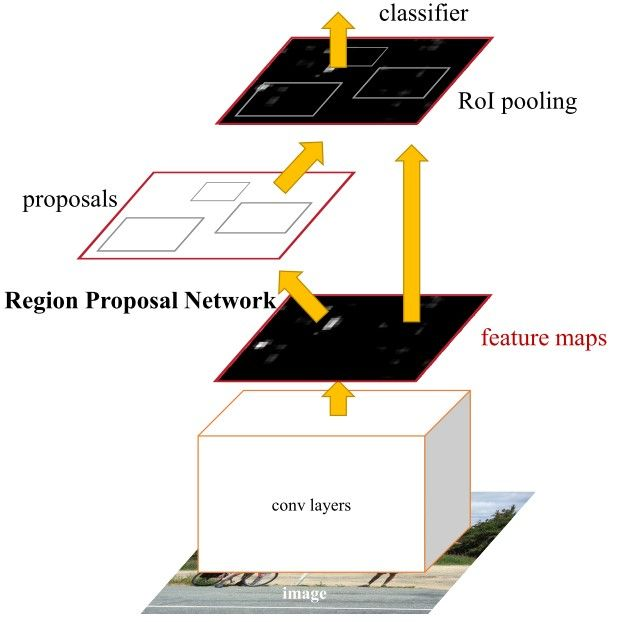
\includegraphics[width=0.6\linewidth]{img/R-CNN.png}
                \caption{Pipeline of Faster R-CNN}
            \end{figure}
        \subsubsection{Region Proposal Generation}
            The RPN module is responsible for generating region proposals. It applies the concept of attention in neural networks, so it guides the Fast R-CNN detection module to where to look for objects in the image. \\ 
            \vspace{3mm}
            The network slides over the conv feature map and fully connects to an n×n spatial window. A low-dimensional vector (512-dimensional for VGG16) is obtained in each sliding window and fed into two sibling FC layers, namely, box-classification layer (cls) and box-regression layer (reg). This architecture is implemented with an n × n conv layer followed by two sibling 1 × 1 conv layers. To increase nonlinearity, ReLU is applied to the output of the n × n conv layer. \\ 
            \vspace{3mm}
            The cls layer outputs a vector of 2 elements for each region proposal. If the first element is 1 and the second element is 0, then the region proposal is classified as background. If the second element is 1 and the first element is 0, then the region represents an object. In other words, it represents a binary classifier that generates the objectness score for each region proposal. \\ 
            \vspace{3mm}
            RPN produces better region proposals compared to generic methods like Selective Search and EdgeBoxes, which are implemented in RCNN and Fast - RCNN. \\ 
            \vspace{3mm}
            The RPN processes the image using the same convolutional layers used in the Fast R-CNN detection network. Thus, the RPN does not take extra time to produce the proposals compared to the algorithms like Selective Search and reduce training time as the RPN and the Fast R-CNN can be merged into a single network.
            \begin{figure}[H]
                \centering
                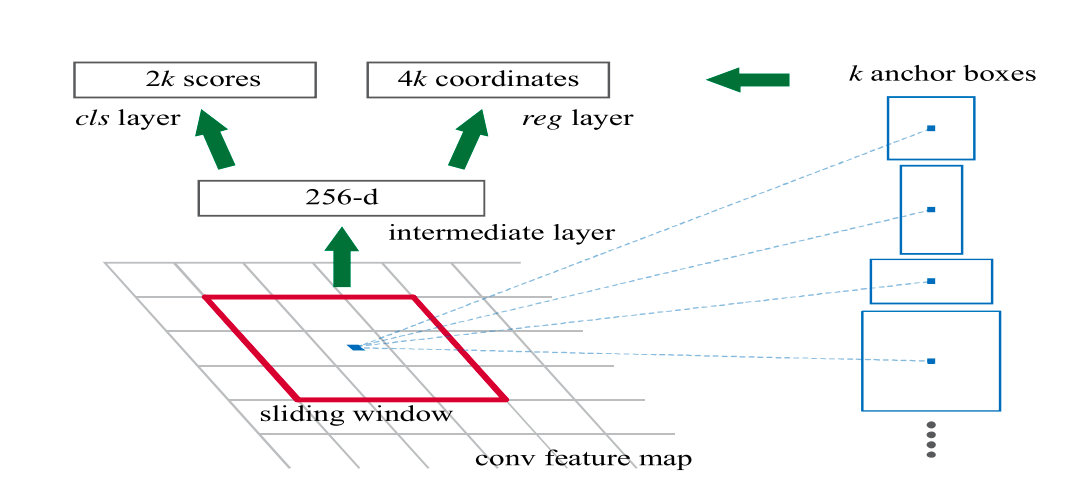
\includegraphics[width=0.6\linewidth]{img/RPN.png}
                \caption{Architecture of RPN}
            \end{figure}
        \subsubsection{Detection Head}
            \begin{enumerate}
                \item \textbf{Anchors} \\ 
                    \vspace{3mm}
                    The feature map of the last shared convolution layer is passed through a rectangular sliding window of size n*n where n = 3 for the VGG-16 net. For each window, K region proposals are generated. Each proposal is parametrized according to a reference box which is called an anchor box. The 2 parameters of the anchor boxes are scale and aspect ratio. Anchors of three scales and three aspect ratios are adopted, therefore K regions are produced from each region proposals. The multi-scale anchors are key to share features across the RPN and the Fast R-CNN detection network. \\ 
                    \vspace{3mm}
                    For training the RPN, each anchor is given a positive or negative \textbf{objectness score} based on the Intersection-over Union (IoU). \\ 
                    \vspace{3mm}
                    The next 4 conditions use the IoU to determine whether a positive or a negative \textbf{objectness score} is assigned to an anchor. Based on this, classification label is produced.
                    \begin{itemize}
                        \item An anchor that has an IoU overlap higher than \textbf{0.7} with any ground-truth box is given a positive objectness label.
                        \item If there is no anchor with an IoU overlap higher than \textbf{0.7}, then assign a positive label to the anchor(s) with the highest IoU overlap with a ground-truth box.
                        \item A negative \textbf{objectness score} is assigned to a \textbf{non-positive} anchor when the IoU overlap for all ground-truth boxes is less than \textbf{0.3}. A negative objectness score means the anchor is classified as background.
                        \item Anchors that are neither positive nor negative do not contribute to the training objective.
                    \end{itemize}
                \item \textbf{Loss Function}
                    \begin{align}
                        L(p_i, t_i) = \frac{1}{N_{cls}} \displaystyle\sum_i L_cls(p_i,p_i\ast) + \lambda \frac{1}{N_{reg}} \displaystyle\sum_i p_i\ast L_{reg} (t_i, t_i\ast)   
                    \end{align}
                    \vspace{3mm}
                    Where $p_i$ is the predicted probability of the $i^{th}$ anchor being an object. The ground truth label $p_i\ast$ is 1 if the anchor is positive, otherwise 0. $t_i$ stores four parameterized coordinates of the predicted boudaring box while $t_i\ast$ is related to the ground truth box overlapping with a positive anchor. $L_cls$ is a binary log loss and $L_reg$ is a smoothed $L_1$ loss. These two terms are normalized with the mini-batch size ($N_cls$) and the number of anchor locations ($N_reg$).
            \end{enumerate}
        \subsubsection{Observations}
            \begin{enumerate}
                \item \textbf{Pros} \\
                    \vspace{3mm}
                    With the proposal of Faster R-CNN, region proposal-based CNN architectures for object detection can really be trained in an end-to-end way.
                \item \textbf{Cons} \\
                    \vspace{3mm}
                    However, the alternate training algorithm is very time-consuming and RPN produces object-like regions (including backgrounds) instead of object instances and is not skilled in dealing with objects with extreme scales or shapes.
            \end{enumerate}

    \subsection{SSD}
        \subsubsection{Feature Extraction}
            SSD uses VGG16 to extract feature maps. VGG16 is a convolutional neural network model proposed by K. Simonyan and A. Zisserman from the University of Oxford in the paper “Very Deep Convolutional Networks for Large-Scale Image Recognition”. The model achieves 92.7\% top-5 test accuracy in ImageNet, which is a dataset of over 14 million images belonging to 1000 classes. It was one of the famous model submitted to ILSVRC-2014. It makes the improvement over AlexNet by replacing large kernel-sized filters (11 and 5 in the first and second convolutional layer, respectively) with multiple 3×3 kernel-sized filters one after another. It is one of the most preferred choices in the community for extracting features from images. The configuration of the VGGNet is publicly available and has been used in many other applications and challenges as a baseline feature extractor.
            \begin{figure}[H]
                \centering
                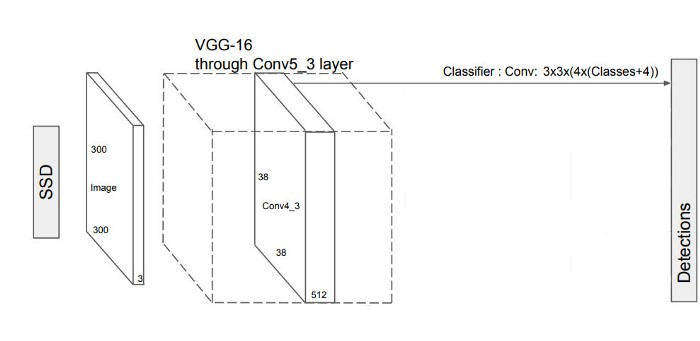
\includegraphics[width=0.6\linewidth]{img/SSD.png}
                \caption{Feature Extractor of SSD}
            \end{figure}
            
            \begin{figure}[H]
                \centering
                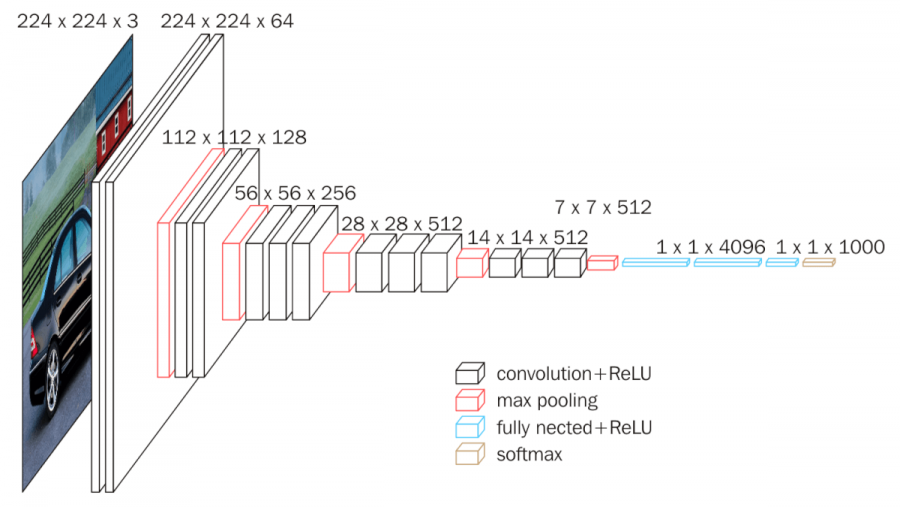
\includegraphics[width=0.6\linewidth]{img/VGG16.png}
                \caption{Architecture of VGG16}
            \end{figure}
        \subsubsection{Multi-scale feature maps for detection}
            Given a specific feature map, instead of fixed grids adopted in YOLO, SSD uses bounding box regression technique,it takes the advantage of a set of default anchor boxes with different aspect ratios and scales to discretize the output space of bounding boxes. To handle objects with various sizes, the network fuses predictions from multiple feature maps with different resolutions. \\ 
            \vspace{3mm}
            SSD adds several feature layers to the end of VGG16 backbone network to predict the offsets to default anchor boxes and their associated confidences. Final detection results are obtained by conducting NMS on multiscale refined bounding boxes.
            \begin{figure}[H]
                \centering
                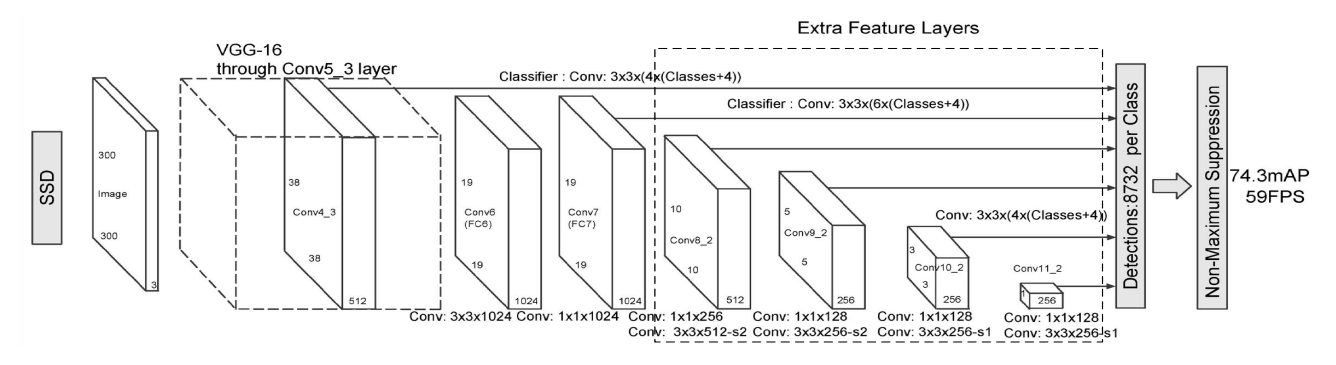
\includegraphics[width=0.6\linewidth]{img/ssd.png}
                \caption{Architecture of SSD}
            \end{figure}
        \subsubsection{Default Boundary Box}
            The default boundary boxes are equivalent to anchors in Faster R-CNN. Default boundary boxes are chosen manually. SSD defines a scale value for each feature map layer. Combining the scale value with the target aspect ratios, we compute the width and the height of the default boxes. For layers making 6 predictions, SSD starts with 5 target aspect ratios: 1, 2, 3, 1/2, and 1/3. Then the width and the height of the default boxes are calculated as:
            \begin{align}
                w = scale.\sqrt{aspect ratio} \\ 
                h = \frac{scale}{\sqrt{aspect ratio}}
            \end{align}
            \vspace{3mm}
            Then SSD adds an extra default box with scale: 
            \begin{align}
                scale = \sqrt{scale.scale at next level}
            \end{align}
            \vspace{3mm}
            Where aspect ratio is equal to 1.
            \begin{figure}[H]
                \centering
                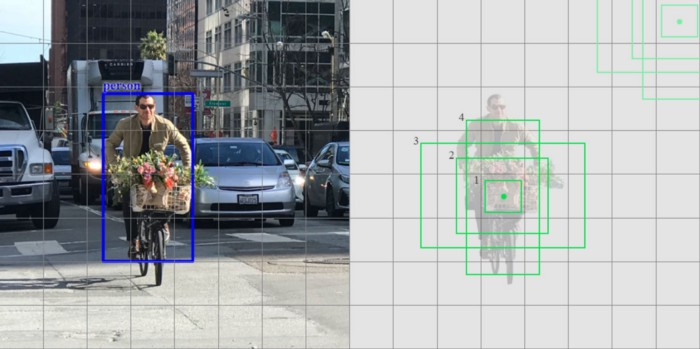
\includegraphics[width=0.6\linewidth]{img/boundary.png}
                \caption{Default Boundary Box}
            \end{figure}
        \subsubsection{Matching Strategy}
            SSD predictions are classified as positive matches or negative matches. SSD only uses positive matches in calculating the localization cost (the mismatch of the boundary box). If the corresponding default boundary box (not the predicted boundary box) has an IoU greater than 0.5 with the ground truth, the match is positive. Otherwise, it is negative. Once we identify the positive matches, we use the corresponding predicted boundary boxes to calculate the cost. This matching strategy nicely partitions what shape of the ground truth that a prediction is responsible for.
            \begin{figure}[H]
                \centering
                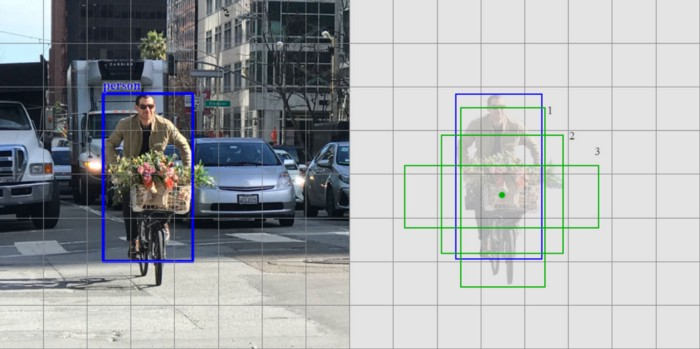
\includegraphics[width=0.6\linewidth]{img/matching.png}
                \caption{Matching with ground truth}
            \end{figure}
        \subsubsection{Loss Function}
            There are two types of loss functions here: Confidence loss and Location loss.
            \begin{itemize}
                \item There are two types of loss functions here: Confidence loss and Location loss. \\
                    \vspace{3mm}
                    The localization loss between the predicted box \textbf{l} and the ground truth box \textbf{g} is defined as the smooth $L_1$ loss with \textbf{$c_x,c_y$} as the offset to the default bounding box \textbf{d} of width \textbf{w} and height \textbf{h}.
                    \begin{align}
                        L_loc(x,l,g) = \displaystyle\sum_{i \in Pos}^{N} \displaystyle\sum_{m \in c_x,c_x,w,h} x_{ij}^k smooth_{L_1} (l_i^m - \hat{g}_j^m) \\ 
                        \hat{g}_j^{c_x} =\frac{(g_j^{c_x} - d_i^{c_x})}{d_i^w} ; \hat{g}_j^{c_y} = \frac{(g_j^{c_y} - d_i^{c_y})}{d_i^h} \\ 
                        \hat{g}_j^w = \log(\frac{g_j^w}{d_i^w}) ; \hat{g}_j^h = \log(\frac{g_j^h}{d_i^h}) \\
                        x_{ij}^p = \left\{ 
                            \begin{array}{ll}
                                1 & \mbox{if IoU > 0.5 between default box i and ground true box j on class p} \\ 
                                0 & \mbox{Otherwise} 
                            \end{array}
                        \right.
                    \end{align} 
                \item The confidence loss is a measure of the confidence that an algorithm quantifies if a bounding box in an image consists of any object or class. For every positive match prediction, we penalize the loss according to the confidence score of the corresponding class. For negative match predictions, we penalize the loss according to the confidence score of the class “0”: class “0” classifies no object is detected.The alpha term balances the contribution of the location losses. The main objective in neural neutral is to analyse the parameters that reduce the loss predictions. \\ 
                    \vspace{3mm}
                    It is calculated as the softmax loss over multiple classes confidences \emph{c} (class score).
                    \begin{align}
                        L_{conf}(x,c) = - \displaystyle\sum_{i \in Pos}^N x_{ij}^p \log(\hat{c}_i^0) where \hat{c}_i^p = \frac{exp(c_i^p)}{(\displaystyle\sum)_p exp(c_i^p)}
                    \end{align}
                    where \emph{N} is the number of matched default boxes.
                \item The final loss function is computed as: 
                    \begin{align}
                        L(x,c,l,g) = \frac{1}{N} (L_{conf}(x,c) + \propto L_{loc}(x,l,g))
                    \end{align}
                    where \emph{N} is the number of positive matches and $\alpha$ is the weight for the localization loss.
            \end{itemize}

        \subsubsection{Hard negative mining}
            SSD still requires negative sampling so it can learn what constitutes a bad prediction. So, instead of using all the negatives, we sort those negatives by their calculated confidence loss. SSD picks the negatives with the top loss and makes sure the ratio between the picked negatives and positives is at most 3:1. This leads to faster and more stable training.

        \subsubsection{Observations}
            \begin{enumerate}
                \item \textbf{Pros} \\ 
                    \vspace{3mm}
                    SSD is a single-shot detector. It has no delegated region proposal network and predicts the boundary boxes and the classes directly from feature maps in one single pass. \\ 
                    \vspace{3mm}
                    To improve accuracy, SSD introduces:
                    \begin{itemize}
                        \item Small convolutional filters to predict object classes and offsets to default boundary boxes.
                        \item Separate filters for default boxes to handle the difference in aspect ratios.
                        \item Multi-scale feature maps for object detection.
                    \end{itemize}
                    \vspace{3mm}
                    SSD can be trained end-to-end for better accuracy. SSD makes more predictions and has better coverage on location, scale, and aspect ratios. With the improvements above, SSD can lower the input image resolution to 300 × 300 with a comparative accuracy performance. Integrating with hard negative mining, data augmentation, and a larger number of carefully chosen default anchors, SSD significantly outperforms the Faster R-CNN in terms of accuracy on PASCAL VOC and COCO while being three times faster.
                \item \textbf{Cons} \\ 
                Shallow layers in a neural network may not generate enough high level features to do prediction for small objects. Therefore, SSD does worse for smaller objects than bigger objects. \\ 
                \vspace{3mm}
                The need of complex data augmentation also suggests it needs a large number of data to train. For example, SSD does better for Pascal VOC if the model is pretrained on COCO dataset.
            \end{enumerate}

    \subsection{YOLO}
        \subsubsection{Network Architecture}
            The whole system can be divided into two major components: Feature Extractor and Detector; both are multi-scale. When a new image comes in, it goes through the feature extractor first so that we can obtain feature embeddings at three (or more) different scales. Then, these features are feed into three (or more) branches of the detector to get bounding boxes and class information.
            \begin{figure}[H]
                \centering
                \includegraphics[width=0.8\linewidth]{img/yolo.png}
                \caption{Major components}
            \end{figure}
        \subsubsection{Feature Extraction}
            The feature extractor YOLO V3 uses is called Darknet-53. Darknet-53 contains 53 layers and borrows the ideas of skip connections to help the activations to propagate through deeper layers without gradient diminishing from ResNet. But the Darknet-53 claims to be more efficient than ResNet101 or ResNet152.
            \begin{figure}[H]
                \centering
                \includegraphics[width=0.8\linewidth]{img/feature_extraction.png}
                \caption{Feature Extraction of YOLOv3}
            \end{figure}
            \vspace{3mm}
            Inside the block, there’s just a bottleneck structure (1x1 followed by 3x3) plus a skip connection. If the goal is to do multi-class classification as ImageNet does, an average pooling and a 1000 ways fully connected layers plus softmax activation will be added. However in the case of object detection, the classification head won't be included, instead, the "detection" head will be added to this feature extractor. Features from last three residual blocks are used in the later detection. 
        \subsubsection{Multi-scale Detector}
            \begin{enumerate}
                \item \textbf{IOU (Intersection Over Union)} \\
                \vspace{3mm}
                Intersection over Union is an evaluation metric used to measure the accuracy of an object detector on a particular dataset. \\
                \vspace{3mm}
                Intersection over Union is a ratio. In the numerator we compute the area of overlap between the predicted bounding box and the ground-truth bounding box The denominator is the area of union, or more simply, the area encompassed by both the predicted bounding box and the ground-truth bounding box. Dividing the area of overlap by the area of union yields our final score — the Intersection over Union. \\
                \vspace{3mm}
                \begin{figure}[H]
                    \centering
                    \includegraphics[width=0.6\linewidth]{img/IOU.png}
                    \caption{IOU formula}
                \end{figure}
                \item \textbf{Anchor Box} \\
                \vspace{3mm}
                The goal of object detection is to get a bounding box and its class. Bounding box usually represents in a normalized xmin, ymin, xmax, ymax format. \\ 
                \vspace{3mm}
                \begin{figure}[H]
                    \centering
                    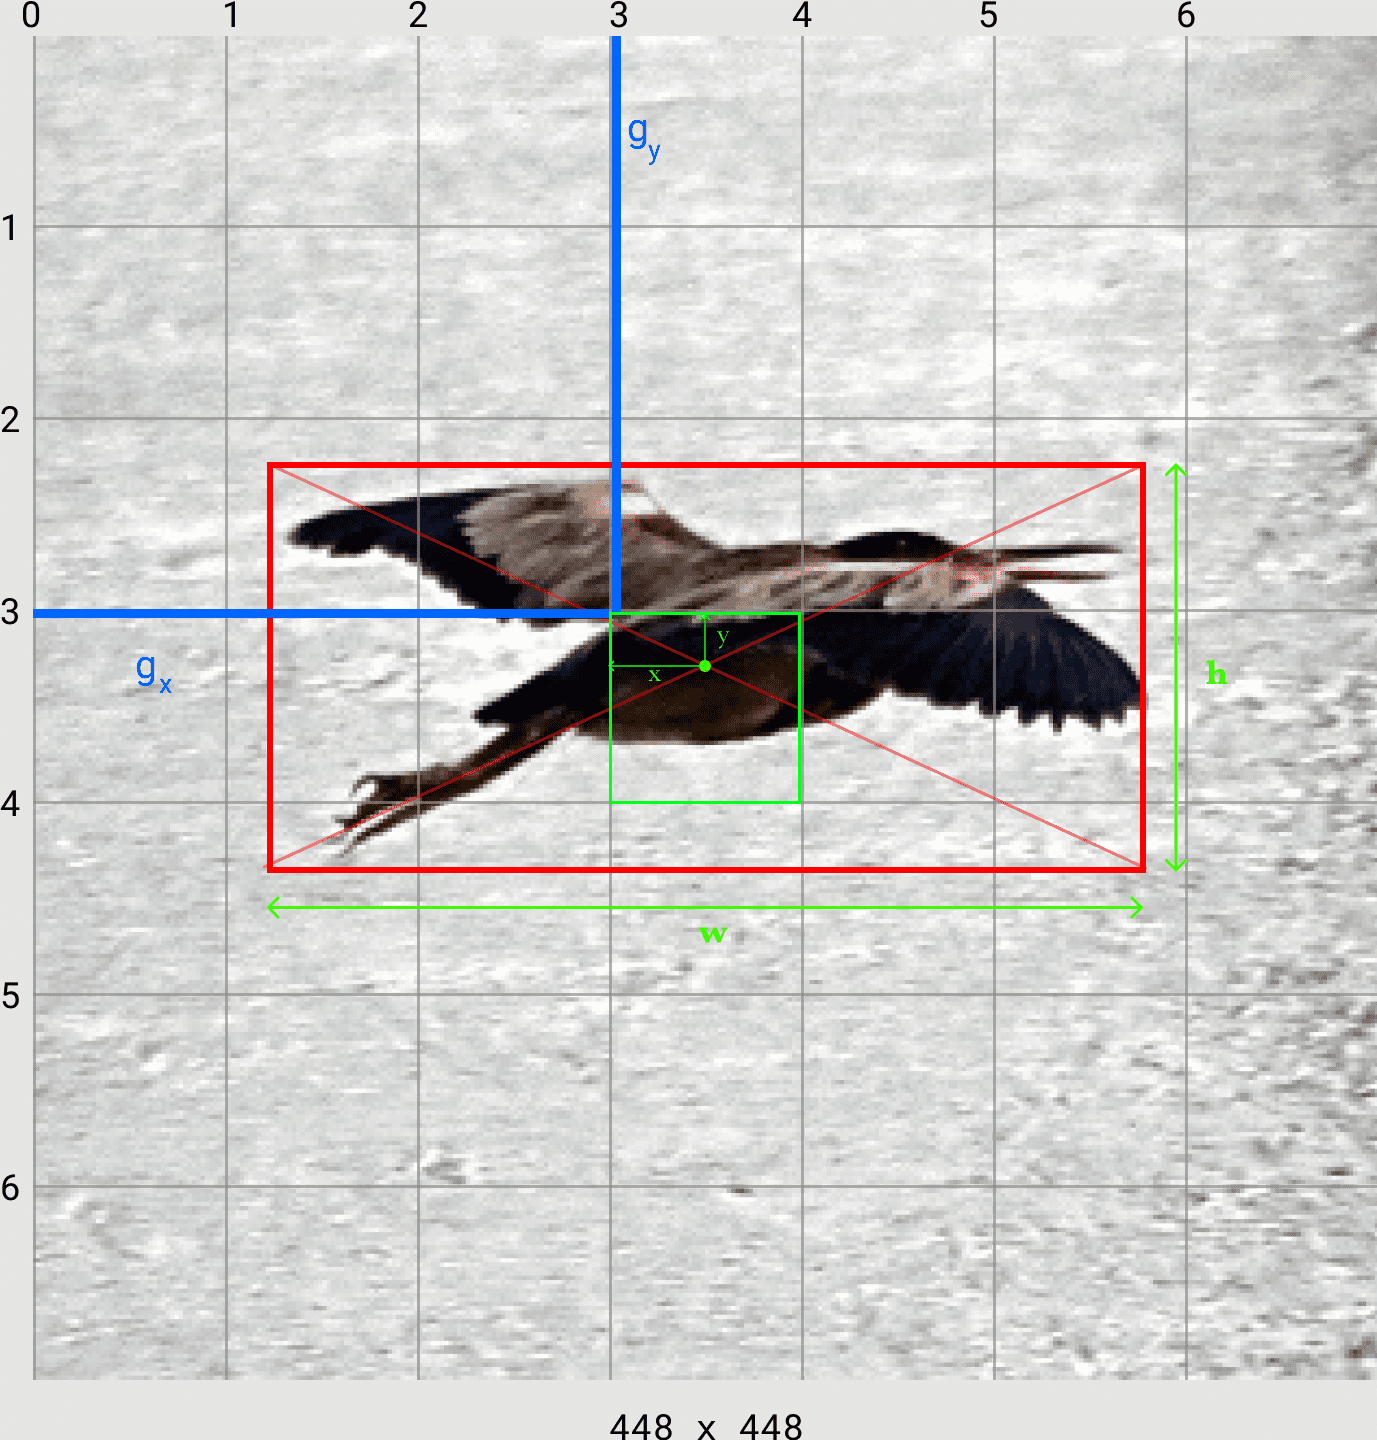
\includegraphics[width=0.6\linewidth]{img/bird.png}
                    \caption{Example for anchor box}
                \end{figure}
                \vspace{3mm}
                The input image is divided into an S x S grid of cells. For each object that is present on the image, one grid cell is said to be “responsible” for predicting it. Anchor boxes are assigned to each cell of the grid.  And once we defined those anchors, we can determine how much does the ground truth box overlap with the anchor box and pick the one with the best IOU and couple them together. \\
                \vspace{3mm}
                In YOLO v3, we have three anchor boxes per grid cell. And we have three scales of grids: \\
                \begin{itemize}
                    \item The location offset against the anchor box: tx,ty,tw,th. This has 4 values.
                    \item The confidence score to indicate if this box contains an object. This has 1 value. The confidence score is defined as $P_{object} * IOU_{pred}^{truth}$ which indicates how likely there is exist objects ($P_{object}\geq0$) and show confidence of its prediction ($IOU_{pred}^{truth}$).
                    \item The conditional class probabilities $P(Class_i|Object)$ to tell us which class this box belongs to. This has number of values according to number of classes.
                \end{itemize}
                \item \textbf{Loss Function} \\
                \vspace{3mm}
                During training the following loss function introduced in YOLO paper is optimize. \\
                \vspace{3mm}
                \begin{align}
                    \lambda_{coord} \displaystyle\sum_{i=0}^{s^2} \displaystyle\sum_{j=0}^{B} \mathbb{1}_{ij}^{obj} [(x_i - \hat{x_i})^2 + (y_i - \hat{y_i})^2] \\
                    \lambda_{coord} \displaystyle\sum_{i=0}^{s^2} \displaystyle\sum_{j=0}^{B} \mathbb{1}_{ij}^{obj} [(\sqrt{w_i} - \sqrt{\hat{w_i}})^2 + (\sqrt{h_i} - \sqrt{\hat{h_i}})^2] \\
                    \displaystyle\sum_{i=0}^{s^2} \displaystyle\sum_{j=0}^{B} \mathbb{1}_{ij}^{obj} (C_i - \hat{C_i})^2 \\ 
                    \lambda_{noobj} \displaystyle\sum_{i=0}^{s^2} \displaystyle\sum_{j=0}^{B} \mathbb{1}_{ij}^{noobj} (C_i - \hat{C_i})^2 \\ 
                    \displaystyle\sum_{i=0}^{s^2} \mathbb{1}_{i}^{obj} \displaystyle\sum_{c \in classes} (p_i(c) - \hat{p_i}(c))^2
                \end{align}
                \vspace{3mm}
                \par The loss function contain 4 parts : centroid loss, anchor box's width and height loss, confidence loss, classification loss. \\
                \vspace{3mm}
                \ding{114}\textbf{Centroid Loss:} the smaller this loss is, the closer the centroids of predictions and ground truth are. Since this is a regression problem, we use mean square error here. Besides, if there're no object from the ground truth for certain cells, we don't need to include the loss of that cell into the final loss. Therefore we also multiple by object mask. Object mask is either 1 or 0, which indicates if there's an object or not. \\ 
                \vspace{2mm}
                \ding{114}\textbf{Anchor's box width and height loss:} this term penalizes the bounding box with inacurate height and width. The square root is present so that erors in small bounding boxes are more penalizing than errors in big bounding boxes. \\ 
                \vspace{2mm}
                \ding{114}\textbf{Confidence loss:} tries to make the confidence score equal to the IOU between the object and the prediction when there is one object or close to 0 when there is no object in the cell. \\ 
                \vspace{2mm}
                \ding{114}\textbf{Classification loss:} is calculated by binary cross-entropy loss. \\
                \vspace{3mm}
                In YOLOv3, they made some modifications to the loss function, confidence loss now uses binary cross-entropy loss to calculated instead of mean square error. The classification loss is now changed into multi-label classification instead of multi-class classification, therefore independent logistic classifiers replaced the softmax for better class prediction.Because some dataset may contains labels that are related to each other.  
            \end{enumerate}
        \subsubsection{Post Processing}
            The final component in this detection system is a post-processor. In YOLO, non maximum suppression is used to eleminate duplicate results.

        \subsubsection{Modifications of YOLO}
            For older version of YOLO, spatial constraint is one major drawback of the algorithm as a grid can analyse only up to two blocks and these two blocks can contain only one class. This results in a reduction in the detection of the nearby objects. It is quite difficult to detect small images in a group image with the help of this algorithm. As it uses the last-stage feature map, which has only the coarse information as it passes through the neural network, the accuracy has a limitation. \\
            \vspace{3mm}
            Bochkovskiy et al proposed the YOLOv4algorithm with significant changes from the previous version, and much better accuracy. Published in April 2020 it is the latest, most advanced iteration of YOLO, and the first developed by the original authors (Redmon et al). To achieve better accuracy, they designed a deeper and complex network, where they used Dense Block. It contains multiple convolutional layers, with batch normalization, ReLU, after which convolution takes place. \\
            \vspace{3mm}
            For the backbone of the feature extraction, they used the CSPDarknet-53, which uses the CSP connections along with Darknet-53 from the previous YOLOv3. Spatial Pyramid Pooling (SPP) is used as the neck over CSPDarknet-53 as it increases the receptive field, differentiates the most significant feature and does not cause a reduction in speed. In place of the Feature Pyramid Network (FPN) in YOLOv3, here they used Path Aggregation Network (PANet). For the head, they used the original YOLOv3 network. \\ 
            \vspace{3mm}
            Apart from the architecture, it consists of a training strategy to get better accuracy without the extra cost to hardware, which is termed as Bag of Freebies. With these, we can get better performance for "free". Another set of strategies which give better results at low cost, but not completely free, were termed as the Bag of Specials. \\ 
            \vspace{3mm}
            With those modification, YOLO is the most commonly used algorithm that is used for detecting natural images as this is the most efficient algorithm for new domains and inputs that are unexpected.
        
    \subsection{Comparision YOLO, SSD and Faster R-CNN}
        \subsubsection{Pascal VOC 2007/2012}
            As YOLO is not skilled in producing object localizations of high IoU, it obtains a very poor result on VOC 2012. However, with the complementary information from Fast R-CNN (YOLO+FRCN) and the aid of other strategies, such as anchor boxes, BN, and fine-grained features, the localization errors are corrected (YOLOv2). 
        \subsubsection{Microsoft COCO}
            Overall, region proposal-based methods, such as Faster R-CNN and R-FCN, perform better than regression/ classification-based approaches, namely, YOLO and SSD, due to the fact that quite a lot of localization errors are produced by regression/classification-based approaches.
        \subsubsection{Time analysis}
            Regression-based models can usually be processed in real time at the cost of a drop in accuracy compared with region proposal-based models. Also, region proposal-based models can be modified into real-time systems.
        \subsubsection{Application in Vehicle Detection System}
            Lecheng Ouyang et al implemented vehicle target detection based on YOLOv3 in complex scenes and showed advantages over traditional target detection algorithms in accuracy and speed. They showed how YOLOv3 can be used for vehicle detection, and it gives an accuracy of 89.16\% at 21fps on the VOC dataset. \\ 
            \vspace{3mm}
            Jeong-ah Kim et al has put three algorithm into test by the the vehicle type classification for the vehicle type recognition was based on the classification of the Korea Expressway Corporation. They found out that Faster R-CNN may not suitable for real-time application, SSD's accuracy is low and sometimes fails to detect a vehicle while YOLOv4 yeilds the most efficient results.[7] \\ 
        \subsubsection{Other Experiments}
            Deepa et al compared all three models for real-time tennis ball tracking and from their work, they concluded that SSD is much efficient and comparatively more accurate accurate algorithm with less computation speed for this particular task of detecting the tennis ball tosses. It worth noticing that, the YOLO version they used is version 1, which performs badly with small objects like tennis ball. This is no longer a shortage to the latest version of YOLO [6]. \\ 
            \vspace{3mm}
            According to [**], when they compared the YOLOv3 algorithm with the SSD, it was shown by evaluation that YOLOv3 had better performance than SSD. If the SSD has an input resolution at 300*300, it would have the same inference as the YOLOv3 at the input resolution 416*416, the precision of YOLOv3 is higher. YOLOv3 is faster than SSD, which is applicable to real-time. \\ 
        
        \subsubsection{Conclusion}
            Choosing YOLOv4 for ITS system is considered most efficient choice so far, therefore we use YOLOv4 to operate as a detector for our system.
\section{Metrics and Evaluations}
    \subsection{Average Precision(AP) and Mean Average Precision(mAP)}
        \begin{itemize}
            \item Recall is the Ratio of the correct predictions and the total number of correct items in the set. It is expressed as percentage of the total correct(positive) items correctly predicted by the model. In other words, recall indicates how good is the model at picking the correct items.
        \end{itemize}
        \begin{align}
            Recall = \frac{TP}{TP + FN}
        \end{align}
        \begin{itemize}
            \item Precision is measured over the total predictions of the model. It is the ratio between the correct predictions and the total predictions. In other words, precision indicates how good the model is at whatever it predicted.
                \begin{align}
                    Precision = \frac{TP}{TP + FP}
                \end{align}
            \item To get True Positives(TP) and False Positives(FP), we use IoU. Using IoU, we now have to identify if the detection(a Positive) is correct(True) or not(False). The most commonly used threshold is 0.5 — i.e. If the IoU is greater than 0.5, it is considered a True Positive, else it is considered a false positive. The COCO evaluation metric recommends measurement across various IoU thresholds, but for simplicity, we will stick to 0.5, which is the PASCAL VOC metric.
            \item Since every part of the image where we didn't predict an object is considered a negative, measuring “True” negatives(TN) is a bit futile. So we only measure “False” Negatives(FN) ie. the objects that our model has missed out.
            \item The average precision (AP) is a way to summarize the precision-recall curve into a single value representing the average of all precisions. The AP is calculated according to the next equation. Using a loop that goes through all precisions/recalls, the difference between the current and next recalls is calculated and then multiplied by the current precision. In other words, the AP is the weighted sum of precisions at each threshold where the weight is the increase in recall.
                \begin{align}
                    AP = \sum_{n=0}^{k=n-1} [Recalls(k) - Recalls(k + 1)] * Precisions(k) \\
                    Recalls(n) = 0, Precisions(n) = 1, n = number\:of\:thresholds.
                \end{align}
        \end{itemize}
        \begin{itemize}
            \item The mean Average Precision or mAP score is calculated by taking the mean AP over all classes and/or overall IoU thresholds, depending on different detection challenges that exist.
                \begin{align}
                    AP = \frac{1}{n} \sum_{n=1}^{k=n} AP_k \\
                    AP_k = the\:AP\:of\:class\:k, n = the\:number\:of\:classes 
                \end{align}
        \end{itemize}
